\documentclass[10pt]{exam}
\usepackage[phy]{template-for-exam}
\usepackage{tikz}
\usetikzlibrary{arrows.meta}

\title{title}
\author{Rohrbach}
\date{\today}



\newcommand{\drawscantron}[2]{
  \begin{center}
    \begin{tikzpicture}
      \node[anchor=south west] at (0,0) {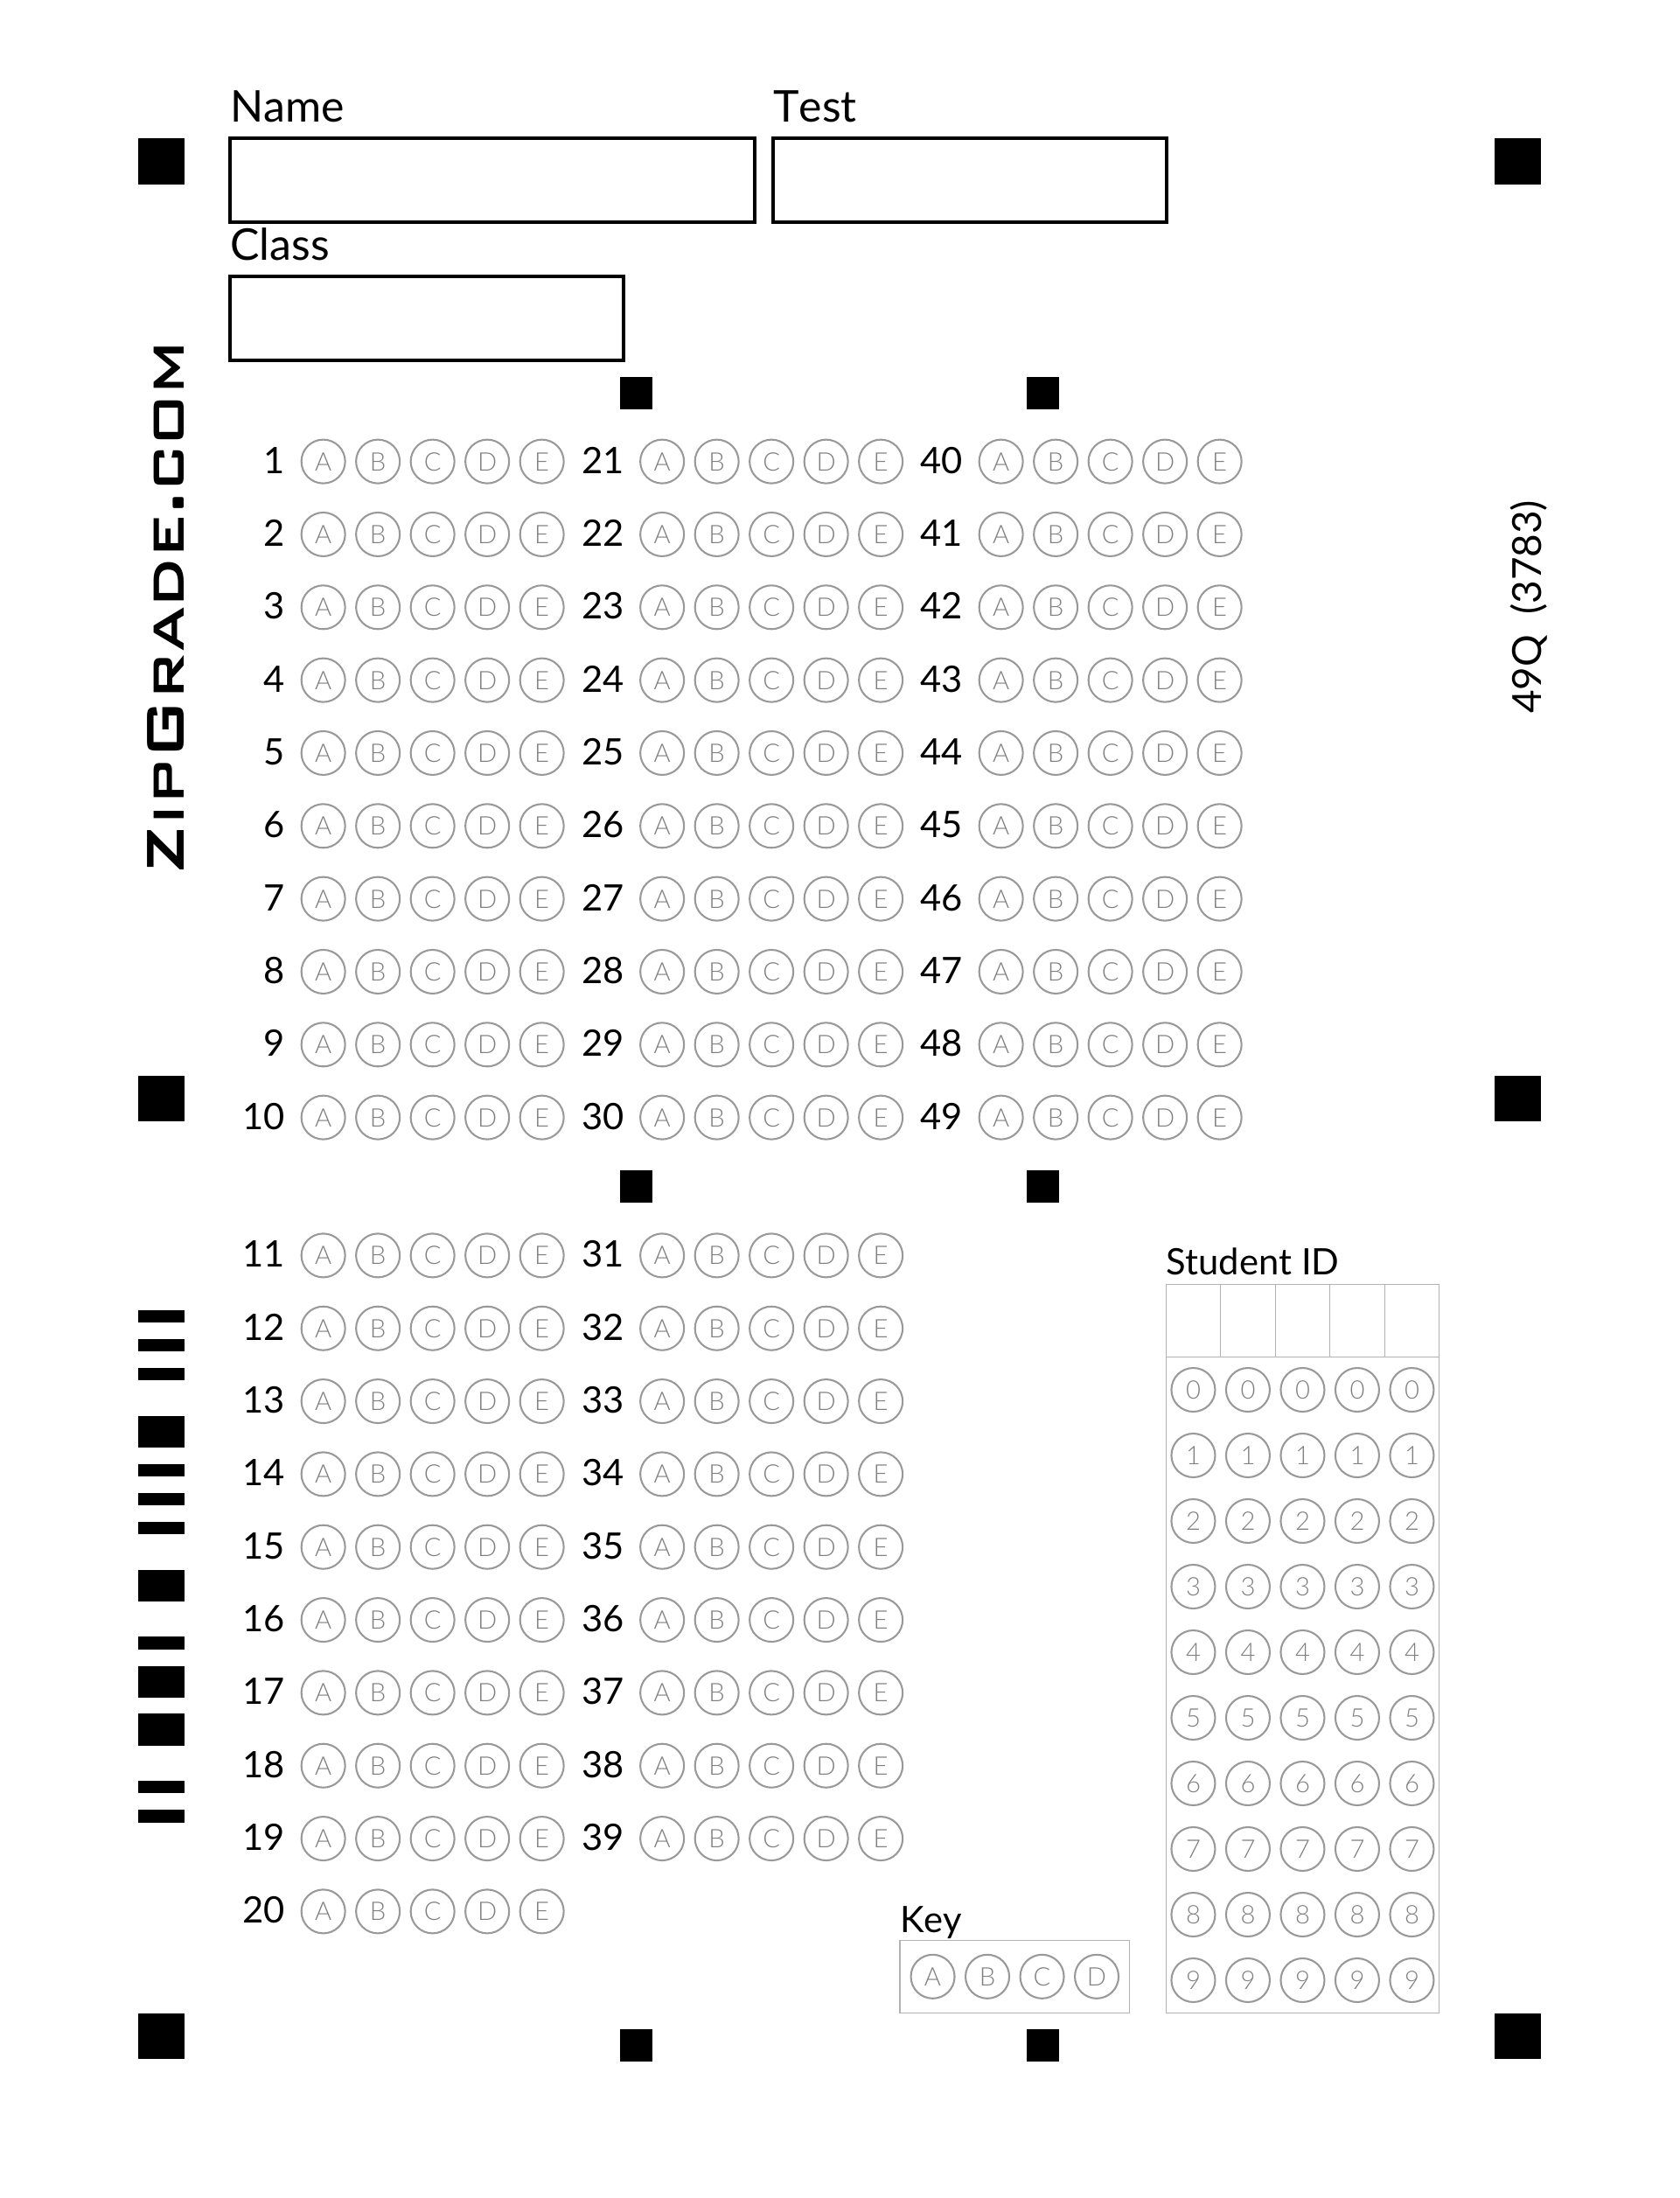
\includegraphics[width=6.4in]{49Q.png}};
      \fill (#1,#2) circle (0.25);
      \node at (9.5,19.5) {Physics Final Exam};
    \end{tikzpicture}

  \end{center}
}

\begin{document}

\newcommand{\printcontent}[1]{
  \vspace*{\stretch{1}}

  \begin{center}
    \Huge 
    
    \textbf{\sc Physics I}

    \textbf{\sc Fall Final Exam}

  \end{center}

  \begin{center}
    \Large (Version #1)
  \end{center}

  \vspace{2em}

  \begin{center}
    
      
\begin{tikzpicture}
        \draw (-0.3,0) -- (0.3,0) -- (0,0.530) -- cycle;
        \node at (0,0.2) {\bf !};
      \end{tikzpicture}
    
    
      {Please do not open this packet until instructed to do so!}
  \end{center}




  \paragraph{Rules} \hfill
  \begin{enumerate}
    \item \textbf{Phones, earbuds, headphones, smartwatches, computers, and other electronics must be put away in your backpacks against the wall during the entirety of the exam.  If electronics are out for \textit{any reason}, you will recieve a zero and a detention!}
    \item Put your name three places: On your Scantron (back of this page), On your Equation Sheet (next page), and on the first page of the Exam Packet.
    \item On your Scantron, bubble in your 3-digit ZipGrade ID from your notebook.
    \item You may write on your equation sheet and on the exam.  There is space provided to show your work, but only your scantron will be graded.
    \item When you are finished, turn in your scantron, equation sheet, and exam packet up front.
    \item Stay silent until all your classmates are finished.  Electronics (especially phones, but also earbuds, headphones, laptops, smartwatches, etc.) need to be kept away until the instructor indicates that everyone is finished.

  \end{enumerate}

  \vs[2]
}

\newcommand{\eqs}{
  {\Huge \bf Equation Sheet}

  \vs

    \begin{center}
    \begin{tabular}{ccc}
      \hline
      \multicolumn{3}{c}{Metric Prefixes}                 \\
      \hline
      \SI{}{\kilo\relax}  & kilo-          & \SI{e3}{}  \\
            --            & (\textit{base})& $10^0$     \\
      \SI{}{\centi\relax} & centi-         & \SI{e-2}{} \\
      \SI{}{\milli\relax} & milli-         & \SI{e-3}{} \\
      \SI{}{\micro\relax} & micro-         & \SI{e-6}{} \\
      \SI{}{\nano\relax}  & nano-          & \SI{e-9}{} \\
      \hline
    \end{tabular}
  \end{center}
%     \vspace*{1em}
%   \end{minipage}





\hrule
\section*{Motion \& Kinematics}

  \subsection*{Constant Velocity \& Acceleration}

      \begin{align*}
          v       &= \frac{d}{t}
        & a       &= \frac{\Delta v}{t}
        &\Delta v &= v_f - v_i
      \end{align*}



  \subsection*{Constant Acceleration}

    \begin{align*}
        v_f   &=  v_i + at 
      & d     &=  v_i t + \frac{1}{2} a t^2
      & v_f^2 &=  v_i^2 + 2 a d \\
      \omit\rlap{\it\footnotesize ``Old Faithful''} &&
      \omit\rlap{\it\footnotesize ``The Big Chalupa''} &&
      \omit\rlap{\it\footnotesize ``Ain't Got No Time''}
    \end{align*}

  \subsection*{Vector Equations}

    \begin{minipage}[b]{.7\linewidth}
      \begin{align*}
        \theta &= \tan^{-1} \left( v_y / v_x \right) &
        v_x^2 + v_y^2 &= v_R^2
      \end{align*}

      \vspace{-2em}

      \begin{align*}
        v_x    &= v_R \cos \left( \theta \right) &
        v_y    &= v_R \sin \left( \theta \right)
      \end{align*}
    \end{minipage}
    %
    \begin{minipage}{.28\linewidth}
      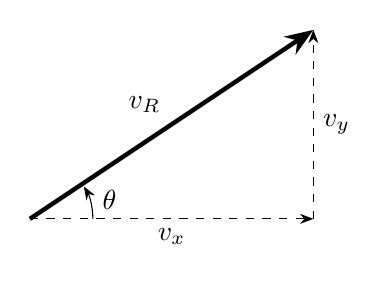
\begin{tikzpicture}[
          component/.append style={
            dashed,
            -{Stealth}
          },
          resultant/.append style={
            ultra thick,
            -{Stealth}
          },
          scale=0.8
      ]
        \draw[resultant] 
                  (0,0) -- (4.5,3) 
                    node[midway,anchor=south east]{\bf $v_R$};
        \draw[component] 
                  (0,0) 
                  -- (4.5,0) 
                    node[midway,anchor=north]{$v_x$} ;
        \draw[component] 
                  (4.5,0)
                  -- (4.5,3) 
                    node[midway, anchor=west]{$v_y$} ;
        \draw[-Stealth] (1,0) node[anchor=south west]{$\theta$}
                  arc[
                    start angle = 0,
                    end angle = 31, 
                    radius = 1
                  ];
      \end{tikzpicture}
    \end{minipage}

    
\hrule
\section*{Forces}

  \begin{align*}
    F_{NET} &=  ma
  & F_{NET} &=  \pm F_1 \pm F_2 \pm \cdots
  & F_G     &=  mg
  & g       &= \SI{9.8}{\meter\per\second^2}
\end{align*}


\hrule
\section*{Circular Motion \& Gravity}

    
    \begin{align*}
        T     &=  \frac{t}{\text{\#rot}}
      & v_T   &=  \frac{2\pi r}{T}
      & v_T   &=  r\omega
      & \omega&= \frac{\text{\#rot}}{t}\times 2\pi
      & F_C   &= \frac{mv_T^2}{r}
    \end{align*}

  \begin{align*}
    F_G &= \frac{Gm_1m_2}{d^2} 
    & G &= \SI{6.67e-11}{\newton\meter^2\per\kilo\gram^2}
  \end{align*}
}


\printcontent{A}
\pagebreak
\drawscantron{9.17}{2.25}
\pagebreak
\eqs
\pagebreak 
\section*{Scratch Work} 
\pagebreak



\printcontent{B}
\pagebreak
\drawscantron{9.67}{2.25}
\pagebreak
\eqs
\pagebreak 
\section*{Scratch Work} 
\pagebreak


\printcontent{C}
\pagebreak
\drawscantron{10.19}{2.25}
\pagebreak
\eqs
\pagebreak 
\section*{Scratch Work} 
\pagebreak


\printcontent{D}
\pagebreak
\drawscantron{10.72}{2.25}
\pagebreak
\eqs
\pagebreak 
\section*{Scratch Work} 





\end{document}